\section{Choosing the standard}\label{sect:cts}

It was important to us to choose an approved standard when implementing an open and free to use solution. If anyone is to rely on the tool we create they must be able to trust that it gives results at least close to that of other tools you can purchase. Selecting one of the models standardized through VQEG testing was therefore a natural choice. After taking that decision we had to choose between a NR, RR and FR model. To date no NR models have been standardized, as shown in section~\ref{sect:history}, which makes it easy to dismiss any such models. The choice between RR and FR models has come came down to choosing the open standard that can be implemented without paying royalties, while also having performed very well in testing. We have chosen OPTICOMs PEVQ model which was standardized in ITU-T Rec. J.247\cite{j.247}. Three other models were also available in this standard, but the OPTICOM model scored overall best which can be seen in table \ref{table:vgaTable}, \ref{table:cifTable} and \ref{table:qcifTable}. The tables use values from the J.247 standard, where the correlation values represent how closely the results from each model correlates with subjective test results. The closer to 1 the correlation value is, the better is the result.


\begin{table}[h]
    \center
    \caption{VGA resolution}
    \begin{tabular}{llllll}
    VGA resolution   & NTT   & OPTICOM & Psytechnics & Yonsei & PSNR  \\
    Avg. correlation & 0.786 & 0.825   & 0.822       & 0.805  & 0.713 \\
    Min. Correlation & 0.598 & 0.685   & 0.565       & 0.612  & 0.499 \\
    \end{tabular}  
     \label{table:vgaTable}
\end{table}

\begin{table}[h]
    \center
    \caption{CIF resolution}
    \begin{tabular}{llllll}
    CIF resolution   & NTT   & OPTICOM & Psytechnics & Yonsei & PSNR  \\
    Avg. correlation & 0.777 & 0.808   & 0.836       & 0.785  & 0.662 \\
    Min. Correlation & 0.675 & 0.695   & 0.769       & 0.712  & 0.440 \\
    \end{tabular}
    \label{table:cifTable}
\end{table}

\begin{table}[h]
    \center
    \caption{QCIF resolution}
    \begin{tabular}{llllll}
    CIF resolution   & NTT   & OPTICOM & Psytechnics & Yonsei & PSNR  \\
    Avg. correlation & 0.819 & 0.841   & 0.830       & 0.756  & 0.662 \\
    Min. Correlation & 0.711 & 0.724   & 0.664       & 0.587  & 0.540 \\
    \end{tabular}
    \label{table:qcifTable}
\end{table}

The biggest limitation of the PEVQ model from ITU-T Rec. J.247 is the tested resolutions which are limited to VGA, CIF and QCIF. HD resolution is Today in full use in most applications, and choosing a standard which is not designed for HD seems strange. This is unfortunately a limitation we have to accept as the models described in newer standards, such as ITU-T Rec. J.341, that does support HD, have been patented in such a way that we cannot make our own implementation for free. 

\subsection{Description of PEVQ}\label{sect:pevq}
PEVQ as standardized in ITU-T Rec. J.247 is a FR objective video quality assessment model designed to measure video quality on mobile and multimedia platforms. It does so by calculating five indicators, each operating in different domains (temporal, spatial, luminance and chrominance) motivated by the human visual system (HVS) so that it may attempt to see the video as a human subject would. The model requires two input signals, the full reference (source) signal and the full degraded signal. The model will go through several stages where both signals are processed and results from the processing stages are weighted together to provide the final result.

\begin{figure}[h]
	  \centering
	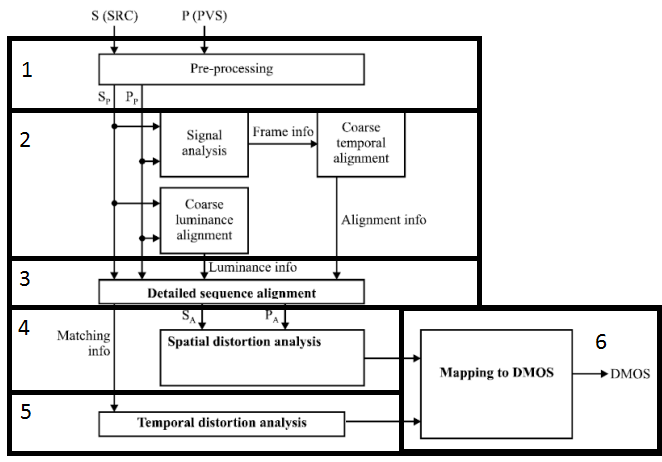
\includegraphics[width=0.7\textwidth,natwidth=662,natheight=588]{images/pevqOverview.png}
	\caption{Overview of the PEVQ model.}
	\label{fig:pevqOverview}
\end{figure}
	  
Using figure~\ref{fig:pevqOverview} we describe the basic flow of PEVQ. The first stage consists pre-processing where a spatial region of interest (RIO) is extracted from the two signals. The RIO is the area on the video where all the following processing will be performed, while the leftover edges are used only for certain calculations where neighbour pixel-data is required. Following the RIO extraction comes a coarse alignment registration of the input sequences which in step 3 is used to perform the detailed sequence alignment that compensates for shifts in the spatial domain. The resulting values from step 3, named \enquote{matching info}, are used to find the perceptual impact of temporal degradations. We will also have the final cropped and aligned versions of the two signals after this stage.

In stage 4 the perceptual difference in the spatial domain between the two signals is processed, providing four distortion indicators. The matching info from stage 3 is further analysed in stage 5 to create one indicator that represents temporal distortions. 

In stage 6 the five main indicators from the previous calculations are weighted together to create the final score. As described in the standard, the final result correlates highly with a mean opinion score (MOS) obtained from subjective tests. It is important to remember that MOS is a widely used term, and there is no definition on what range of values a MOS score must be within. MOS simply represents a scale with which we can give a meaningful score. A description of various ways to use MOS can be found in \cite{p800}. To get a deeper understanding of how PEVQ does its analysis, please see the J.247 publication in\cite{j.247}.
